% !TEX root = BA-Bericht.tex
\chapter{Realisierung}
% TODO Beschreibung der Umsetzung der definierten Ziele, einschliesslich der aufgetretenen Schwierigkeiten und Einschränkungen

% Dies ist das Hauptkapitel Ihrer Arbeit! Hier wird die Umsetzung der eigenen Ideen und Konzepte
% (Kapitel 3) anhand der gewählten Methoden (Kapitel 4) beschrieben, inkl. der dabei aufgetretenen
% Schwierigkeiten und Einschränkungen.

\section{Projektmanagement}

\subsection{Meilenstein 1: Grobkonzept}

\subsection{Meilenstein 2: Zwischenpräsentation}

\subsection{Resultate}

Die folgende Tabelle~\fullref{tab:resultate} beschreibt alle Resultate und Unterresultate die während dieser Bachelorarbeit erstellt werden.
Diese Tabelle wurde zusammengestellt anhand der Anforderungen im Abschnitt~\ref{sec:Anforderungen}.

Jedes Resultat hat einen eindeutigen Identifier in  der Spalte ''Nr'' aufgelistet.
Die Spalte ``Anforderung'' bezieht sich darauf, welche Anforderungen für das jeweilige Resultat massgebend sind.
In der letzten Spalte ''Geschätzter Arbeitsaufwand'', wurde zu beginn des Projekts abgeschätzt wie viel Arbeitsaufwand (in Stunden) das Resultat verursacht.

\begin{longtable}{p{0.8cm} l p{3.5cm} p{2cm}}
    \toprule
    \bfseries Nr & \bfseries Resultat & \bfseries Anforderung& \multicolumn{1}{p{3cm}}{\bfseries Geschätzter Arbeitsaufwand} \\
    \midrule \endhead
    D            & \textbf{Dokumentation}                                       & \reqref{DOCS} & \textbf{Total 44h}  \\
    \midrule                                                               
    D.1          & \; Dokumenten Layout                                &       & 8h   \\
    D.2          & \; Aufbau des Berichts                              &       & 4h   \\
    D.3          & \; Titelseite                                       &       & 2h   \\
    D.4          & \; Zusammenfassung / Abstract                       &       & 2h   \\
    D.5          & \; Einleitung                                       &       & 4h   \\
    D.6          & \; Beschreibung Motivation / Problem                &       & 2h   \\
    D.7          & \; Beschreibung der Aufgabenstellung                &       & 2h   \\
    D.8          & \; Beschreibung der Ziele / Vision                  &       & 1h   \\
    D.9          & \; Fragestellungen / Hypothesen                     &       & 2h   \\
    D.11         & \; Reflektion / Fazit                               &       & 3h   \\
    D.12         & \; Persönliches Projektfazit                        &       & 1h   \\
    D.13         & \; Ausblick                                         &       & 4h   \\
    D.14         & \; Anhang                                           &       & 3h   \\
    D.15         & \; Zwischenpräsentation                             & \reqref{PRES}  & 6h  \\
    \midrule                                                               
    R            & \textbf{Research State of the Art}                           & \reqref{SDTF} \reqref{DOCS}  & \textbf{Total 40h} \\
    \midrule                                                               
    R.1          & \; Literatur sammeln (Recherche)                    &       & 12h  \\
    R.2          & \; Bibliographie erstellen                          &       &  4h  \\
    R.3          & \; P2P Networks                                     &       &  2h  \\
    R.3.1        & \;   - Latenz / Bandbreite / Performanz             &       &  2h  \\
    R.4          & \; Beschreibung I2P                                 &       & 10h  \\
    R.4.1        & \; -- Begrifflichkeiten                              &       &  4h  \\
    R.4.2        & \; -- Funktionsweise                                 &       &  2h  \\
    R.4.3        & \; -- Bandbreite                                     &       &  2h  \\
    R.4.4        & \; -- Latenz                                         &       &  2h  \\
    R.5          & \; Deployment von Testnetzwerken                    &       &  4h  \\
    R.6          & \; Beschreibung der Wissenschaftlichen Methode      &       &  2h  \\
    R.7          & \; Metriken für die Auswertung                      & \reqref{TPER} \reqref{TISO} \reqref{TREP}  &  6h  \\
    \midrule                                                               
    K            & \textbf{Testkonzept          }                               & \reqref{TKON} \reqref{DOCS}  & \textbf{Total 46h}  \\
    \midrule                                                               
    K.1          & \; Beschreibung Ideen / Konzepte                    &       &  4h  \\
    K.2          & \; Anforderungen an den Teststand                   &       &  4h  \\
    K.3          & \; Teststrategie                                    &       &  4h  \\
    K.4          & \; Architektur Teststand                            &       &  4h  \\
    K.5          & \; Komponentendiagramm                              &       &  2h  \\
    K.6          & \; Beschreibung was gemessen werden soll            &       &  8h  \\
    K.7.1        & \; -- Bandbreite                                     & \reqref{TLIM} &  2h  \\
    K.7.1        & \; -- Anzahl Tunnels                                 & \reqref{TCNF}    &  2h  \\
    K.7.1        & \; -- Latenz von Nachrichten                         & \reqref{TLAT}    &  2h  \\
    K.7.1        & \; -- Ressourcenauslastung eines Knotens             & \reqref{TPER}    &  2h  \\
    K.8          & \; Beschreibung wie gemessen wird                   &       & 10h  \\
    K.8.1        & \; -- Isolation des Netzwerks                        & \reqref{ORDR}    &  2h  \\
    K.8.1        & \; -- Verschiedene Netzwerksegmente                  & \reqref{ORDR}    &  2h  \\
    K.8.2        & \; -- Latenz                                         & \reqref{ORDR}    &  2h  \\
    K.8.3        & \; -- Bandbreite                                     &       &  2h  \\
    K.8.4        & \; -- Konfigurationsmöglichkeiten                    & \reqref{TCNF} &  2h  \\
    K.9.5        & \; \glsname{ci}                                     & \reqref{TVRS} &  6h  \\
    K.9.6        & \; Beschreibung der Auswertungsmethode              &               &  4h  \\
    \midrule                                                               
    S            & \textbf{Teststand Design und Implementation}                 & \reqref{TINF} \reqref{DOCS} & \textbf{Total 124h} \\
    \midrule
    S.1          & \; Software Design                                  &       &  16h \\
    S.1          & \; Implementation                                   &       &  72h \\
    S.2.1        & \; -- Deployment des Testnetzwerkes                  & \reqref{TVRS} \reqref{TPER} &  8h \\
    S.2.2        & \; -- Netzwerksegmentierung                          & \reqref{TISO} &  8h \\
    S.2.3        & \; -- Konfigurationsmöglichkeiten                    & \reqref{TCNF} &  8h \\
    S.2.4        & \; -- Skalierung                                     & \reqref{TSCL} &  8h \\
    S.2.5        & \; -- Bandbreitenbeschränkung                        & \reqref{TLIM} &  8h \\
    S.2.6        & \; -- Reproduzierbarkeit                             & \reqref{TREP} &  8h \\
    S.2.7        & \; -- Latenzmessung                                  & \reqref{TLAT} &  8h \\
    S.2.8        & \; -- Messung der Ressourcenauslastung               & \reqref{TPER} &  8h \\
    S.2.9        & \; -- Verschiedene Testaufbauten                     & \reqref{TVRS} &  8h \\
    S.3          & \; Test des Labors                                  &       &  24h \\
    S.4          & \; Handbuch für den Teststand                       &       &  12h \\
    S.4.1        & \; -- Installation                                   &       &   2h \\
    S.4.3        & \; -- Konfiguration                                  &       &   2h \\
    S.4.3        & \; -- Ausführen von Messungen                        &       &   2h \\
    S.4.3        & \; -- Beschreibung der gesammelten Messdaten         &       &   4h \\
    S.4.3        & \; -- Beispiele                                      &       &   2h \\
    \midrule                                                                        
    A            & \textbf{Messung und Auswertung}                              & \reqref{EVAL} \reqref{DOCS}   & \textbf{Total 52h}  \\
    \midrule
    A.1          & \; Sammlung an Messdaten für die Auswertung         &        &  12h  \\
    A.2          & \; Beschreibung der Auswertungsmethode              &        &   4h  \\
    A.3          & \; Auswertung der Messungen                         &                    & 20h  \\
    A.3.1        & \; -- Einfluss der Knoten auf die Latenz             & \reqref{TLAT}      &  6h  \\
    A.3.2        & \; -- Einfluss der Anzahl Verbindungen auf die Latenz& \reqref{TLAT} \reqref{TLIM} &  6h  \\
    A.3.3        & \; -- Einfluss der Bandbreite auf Latenz             & \reqref{TLAT} \reqref{TLIM} &  6h  \\
    A.3.4        & \; -- Äussere Einflüsse / Unreinheiten               & \reqref{TREP} \reqref{TISO} &  2h  \\
    A.4          & \; Verschiedene Diagramme/Grafiken                  &       &  8h  \\
    A.5          & \; Auswertung der Anforderungen an den Teststand    & \reqref{TINF} &  4h  \\
    A.6          & \; Zusammenfassung der Auswertung                   &       &  4h  \\
    \midrule                                                               
    P            & \textbf{Project Management Dokumentation}                    & \reqref{DOCS} \reqref{ITER}  &  \textbf{Total 54h}  \\
    \midrule
    P.1          & \; Beschreibung Projektorganisation                 &       &  1h  \\
    P.3          & \; Projektmanagement Methode                        &       &  2h  \\
    P.2          & \; Beschreibung Projektumfang                       &       &  2h  \\
    P.4          & \; Projektplanung                                   &       &  8h  \\
    P.5          & \; Liste von Requirements                           &       &  4h  \\
    P.6          & \; Liste von Resultaten                             &       &  4h  \\
    P.9          & \; Arbeitsjournal                                   &       &  4h  \\
    P.10         & \; Meeting-Protokolle und Notizen                   &       & 29h  \\
    \midrule                                                               
                 & \bfseries  Geschätzter Arbeitsaufwand               & \textbf{Total} & \bfseries 360h \\
    \midrule
    \bottomrule
    \caption{Resultate}
    \label{tab:resultate}
\end{longtable}

Diese Liste von Resultaten ist auch ein guter Ausgangspunkt um davon Issues für den Issue-Tracker zu erstellen.
Jeder issue kann nun auch sortiert werden nach Resultat-Kategorien z.B. ''Recherche'', ''Projektmanagement'', ''Dokumentation'', ''Evaluation'', ''Präsentation'', etc.

\newpage

\section{Systemarchitektur}

Grob besteht die entwickelte Software für den Teststand aus drei teilen.

\begin{enumerate}
    \item \textbf{Tester-Software}: Hier ist die Deployment-Konfiguration für die Test-VM zu finden, sowie die verwendeten Tools zur Auswertung.
    \item \textbf{Test-VM:} Hier ist die Konfiguration für das 
    \item \textbf{Testnetzwerk:} Das Testnetzwerk besteht aus i2pd-Containern sowie aus dem Reseed-Container der verwendet wird zum Bootstrapping des Testnetzwerks.
\end{enumerate}

Die Abbildung~\fullref{fig:architektur-diagramm} zeigt in einem Komponenten-Diagram die Systemarchitektur auf.


\begin{landscape}% Landscape page
\begin{figure*}[ht]
  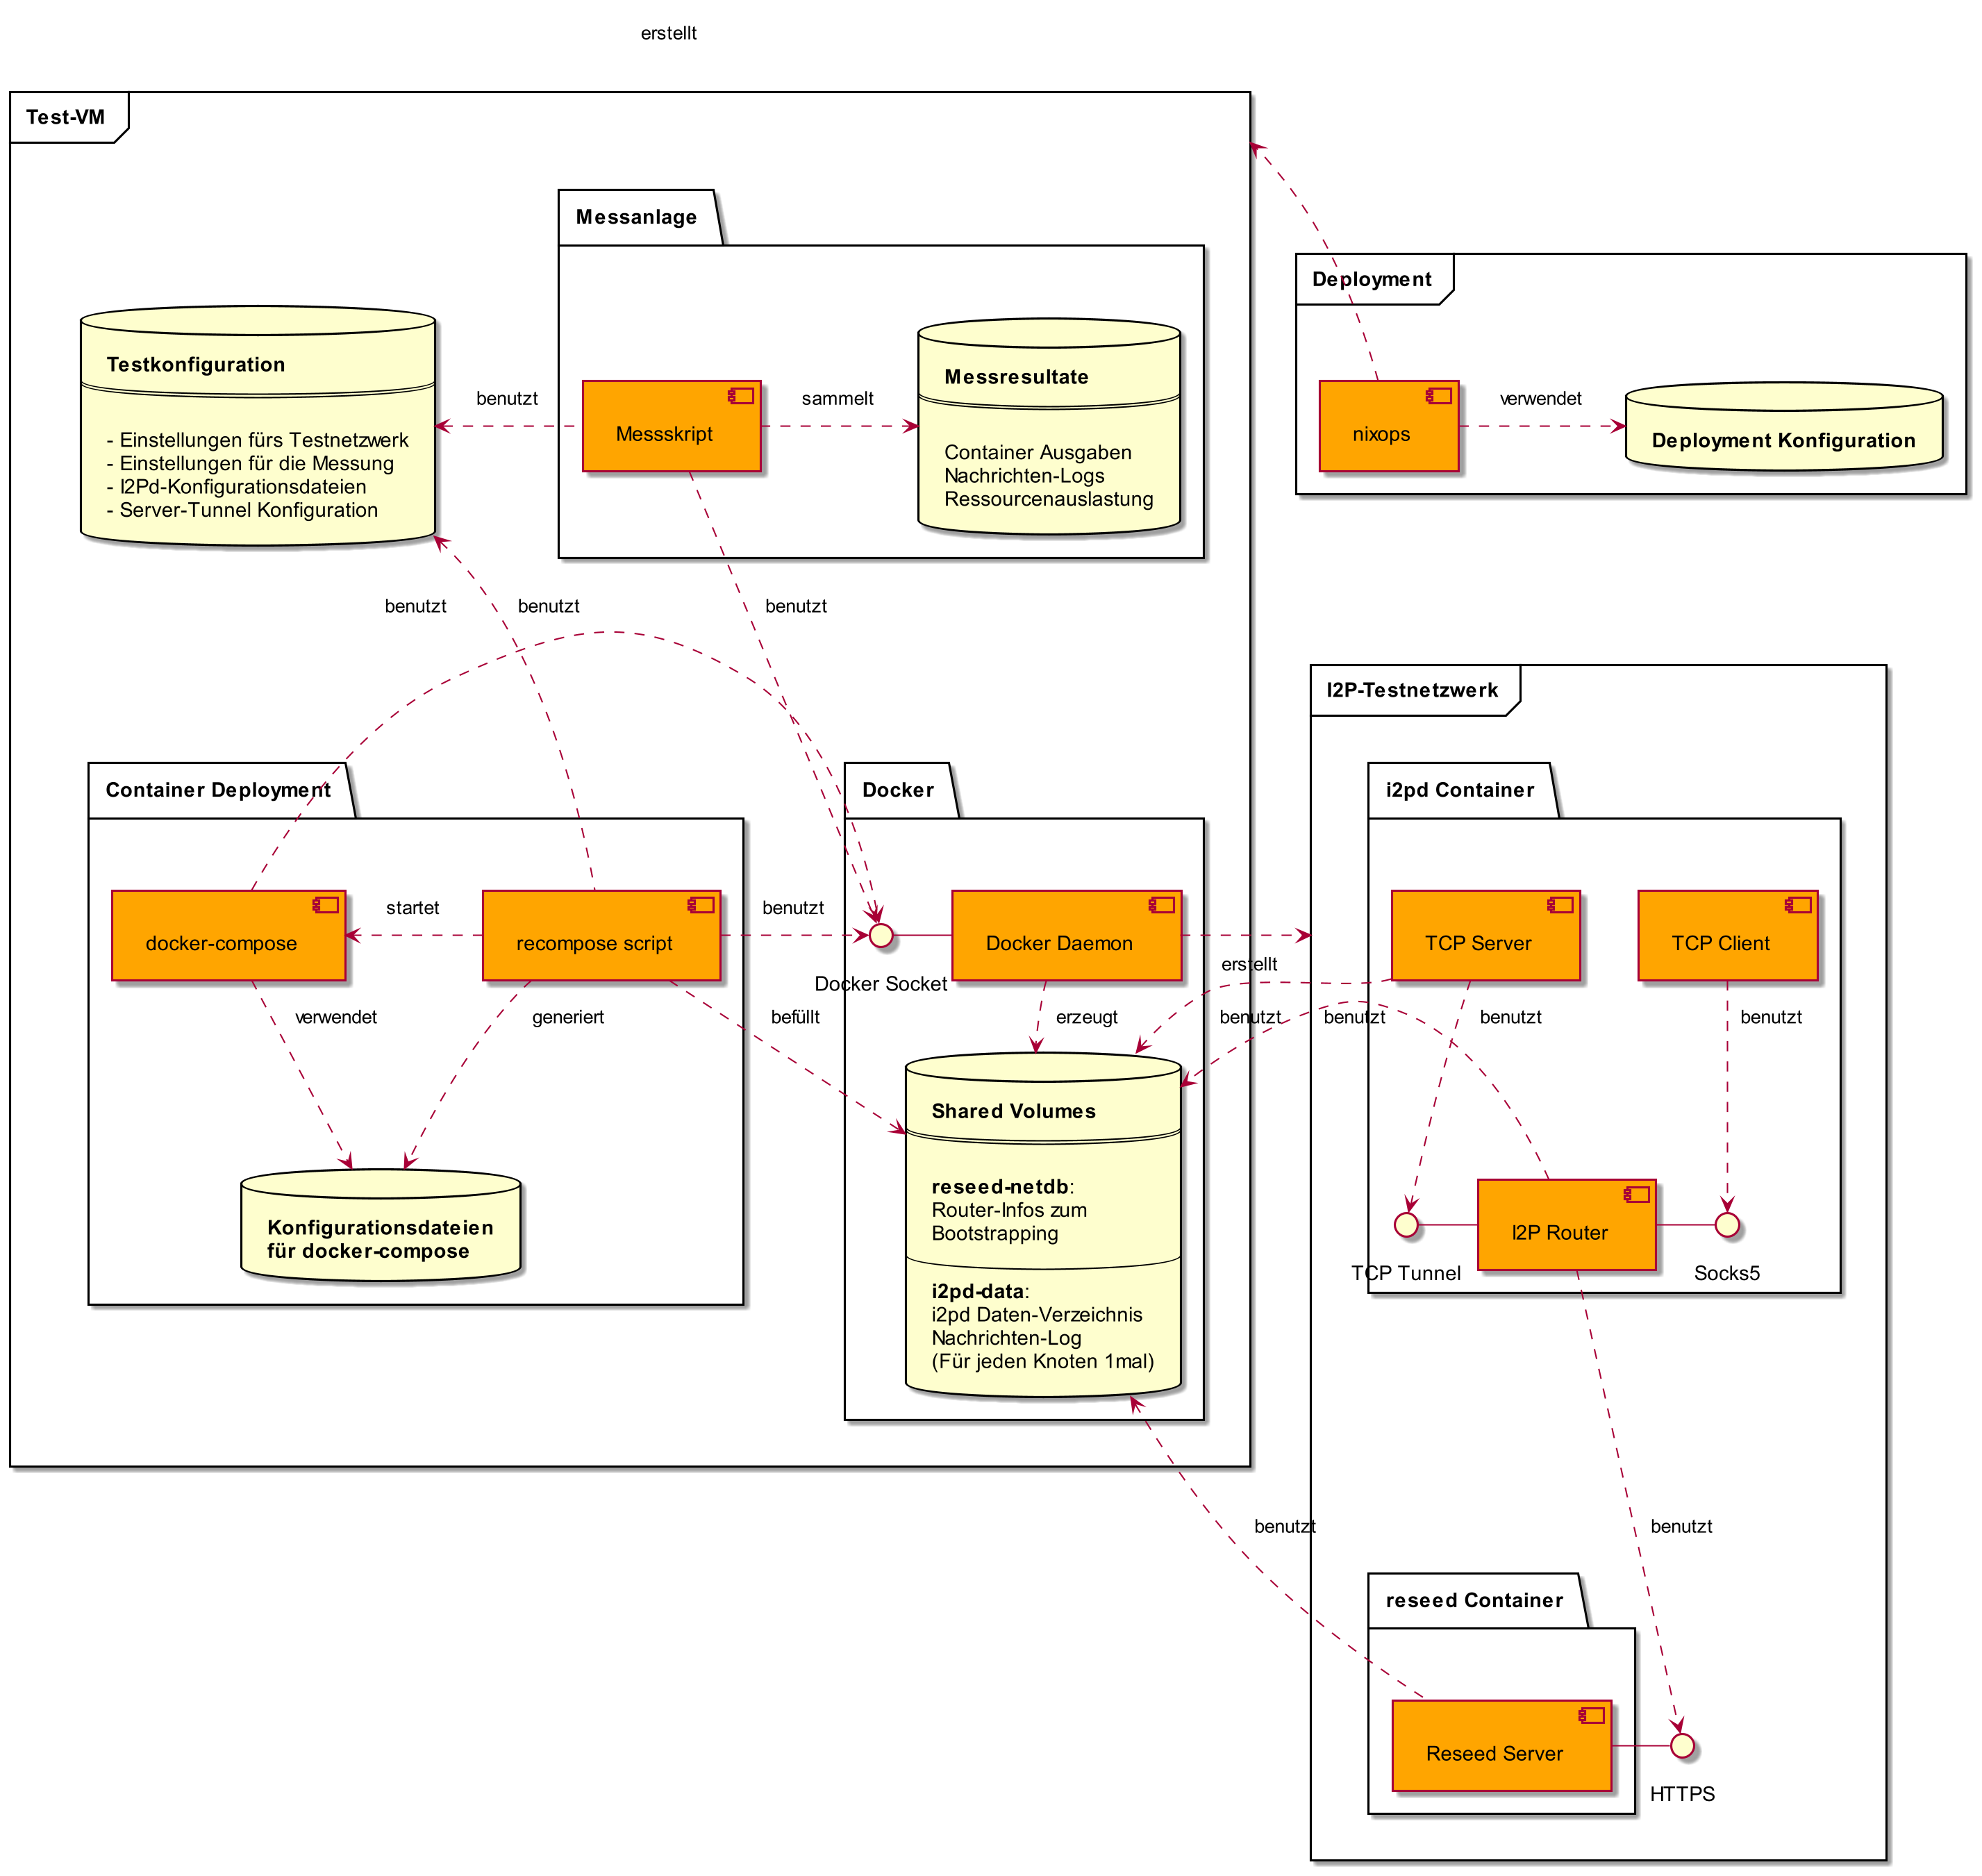
\includegraphics[height=0.85\textwidth]{include/uml/componentDiagram.png}
  \caption{Architektur-Diagramm}\label{fig:architektur-diagramm}
\end{figure*}
\end{landscape}% Landscape page


\section{Komponentendesign}

\subsection{Deployment der Test-VM}

NixOps erlaubt es eine NixOS-Systemkonfiguration auf diverse Arten von Maschinen zu deployen.

\subsection{Konfiguration}

Die Konfiguration für

\subsection{Recompose-Skript}

Das Recompose-Skript ist dafür verantwortlich das Docker-Netzwerk aufzubauen und zu managen.

Als wichtigster Punkt wird hier der 



\subsection{Deployment von der Container}

Da ich bereits NixOps zum deployment der Container verwendet habe, schien es naheliegend die NixOS-Container Technologie zu verwenden.

Jedoch bin ich mit diesem Ansatz an mehreren Stellen an Grenzen gestossen.

Als erstes traten Probleme mit der Netzwerkkonfiguration. Die NixOS-Container implementation scheinte die 

• Erst Probleme mit der Netzwerkkonfiguration
• Probleme mit Docker-Kompatibilität
• Skaliert nicht auf mehr als ein paar dutzend Container. Zu viel
RAM benötigt lediglich zum Berechnen der verschiedenen
Container-Konfigurationen.

Es hat 

Anfangs wurde auf ein Ansatz mit 


\subsection{Skalierung der i2pd-Container}

Der erste Lösungsansatz mit NixOS-Containern hat sich als ungeeignet herausgestellt. \seereq{TSCL}

Dieser Ansatz wurde verworfen, weil dies dazu geführt hat, das die i2pd-Container untereinander nicht kommunizieren konnten.

\subsection{Bootstrapping}

Die I2P-Router im öffentlichem I2P-Netzwerk können sich hier einfach an den öffentlich verfügbaren Reseeder eine \lstinline|su3|-Datei herunterladen.
Diese \lstinline|su3|-Datei beinhaltet RouterInfos. 
Diese RouterInfos beinhalten die nötigen Informationen wie public-key und Netzwerkadresse, um die Kommunikation zu starten.

Im privaten und abgeschotteten Testnetzwerk sind die öffentlichen Reseed-Server jedoch nicht erreichbar.
Deshalb muss ein anderer Weg gefunden werden das private I2P-Netzwerk zu bootstrappen.



Denn der Floodfill-Anstatz entspricht nicht unbedingt der Realität, denn die Reseeder-Knoten können liefern nicht allen I2P-Routern dieselbe Liste an Peers.

Auch kann die Konfiguration des Reseeders eine wichtige Rolle spielen, denn dieser bestimmt mit der Liste an Peers die er den I2P-Routern liefert den Konnektivitätsgrad der Knoten.


\subsection{Konfiguration}

Die Konfiguration des Teststands kann mittels einer json-Konfigurationsdatei einfach angepasst werden.
Diese kann, falls nötig einfach von verschiedenen Orten gelesen werden.

\subsection{Resultate zurücklesen}

Just read logs? Use some Docker cp magic?

\section{Umsetzung / Programmierung}

Der Komplette Quellcode für das Deployment der Test-VM, die Erstellung des Testnetzwerk's und die Messanlage ist im folgenden Repository zu finden:

\url{https://codeberg.org/mkuettel/i2p-testnet}.

\section{Test-VM}

Die Test-VM wurde so umgesetzt, das diese mittels nixops deployed werden kann.

\section{1. Lösungsansatz: NixOS-Container}

NixOS erlaubt es deklarativ Container zu definieren.

% \begin{lstlisting*}[language=nix,label=src:nixos-container,caption=Beispiel wie Nixos Container definiert werden können]
%
%     boot.enableContainers = true;
%     containers = {
%         "container1" = {
%             config = { config, pkgs, ... }:
%                 {
%                     # NixOS system configuration for this container
%                     services.httpd.enable = true;
%                 }
%             # more container settings ... 
%         };
%         # "container2" .... 
%     }
% \end{lstlisting*}

Wichtig dabei ist, dass es sich hierbei nicht um einen Docker-Container, sondern um NixOS-Container handelt.
Im Hintergrund brauchen jedoch beide Container-Arten die gleichen Linux-Kernel-Features (namespaces, cgroups, ... ).


Siehe \lstinline|containers.nix| in der \lstinline|i2p-testnet| Repository für die Effektive implementation

\subsection{Bootstrapping}

Da das Testnetzwerk

\subsubsection{Reseed-Server}

Dieser Ansatz hat den Vorteil, das so das Testnetzwerk schnell aufgebaut werden kann.

Die \lstinline|i2pd|-Implementation beinhaltet selber keinen 

Die Go-Implementation dieses Reseed-Servers ist hier zu finden:

\url{https://codeberg.org/diva.exchange/i2p-tools}

Diese Version basiert auf der folgenden GitHub version:

\url{https://github.com/MDrollette/i2p-tools}

\subsubsection{Ablauf}

Der Bootstrapping-Vorgang im Testnetzwerk wird wie folgt abgehandelt (vgl. mit Abbildung~\fullref{fig:bootstrap-diagram}):

\begin{enumerate}
    \item Erstellen der Container für den Reseed-Sever und den I2P-Knoten
    \item Der Reseed-Server erstellt die nötigen Schlüssel und Zertifikate, um einerseits später den HTTPS-Reseed-Server zu starten und andererseits die su3-Dateien zu signieren.
    \item Der Reseed-Server-Container fängt an zu warten bis er alle RouterInfo's von allen I2P-Knoten erhalten hat
    \item Die I2P-Router werden kurzzeitig gestartet, bis diese Ihre RouterInfo Datei erstellen. Die I2P-Router werden anschliessend wieder gestoppt, da der Reseed-Server im Moment noch nicht in Betrieb ist, da ihm die RouterInfos noch fehlen.
    \item Die I2P-Knoten-Container warten anschliessend bis der HTTPS-Reseed-Server verfügbar ist.
    \item Auf der Test-VM kopiert ein Hintergrund-Job alle RouterInfos vom I2P-Container in die NetDb des Reseed-Server-Containers.
    \item Nach kurzer Zeit hat der Reseed-Server-Container alle benötigten RouterInfos. Nun generiert dieser die su3-Datei aus den RouterInfos und startet anschliessend nun effektiv den HTTPS-Reseed-Server.
    \item Die I2P-Knoten-Container können nun den HTTPS-Reseed-Server erreichen und somit wird der I2P-Router gestartet.
    \item Die I2P-Router laden nun die su3-Datei herunter und können so die anderen Knoten ausfindig machen und Ihre Arbeit starten.
\end{enumerate}

Welche Reseeder ein I2P-Router anfragt, kann mittels der \lstinline|i2pd|-Konfigurationsoption \lstinline|urls| festgelegt werden.


\clearpage
\begin{landscape}% Landscape page
\begin{figure*}[ht]
  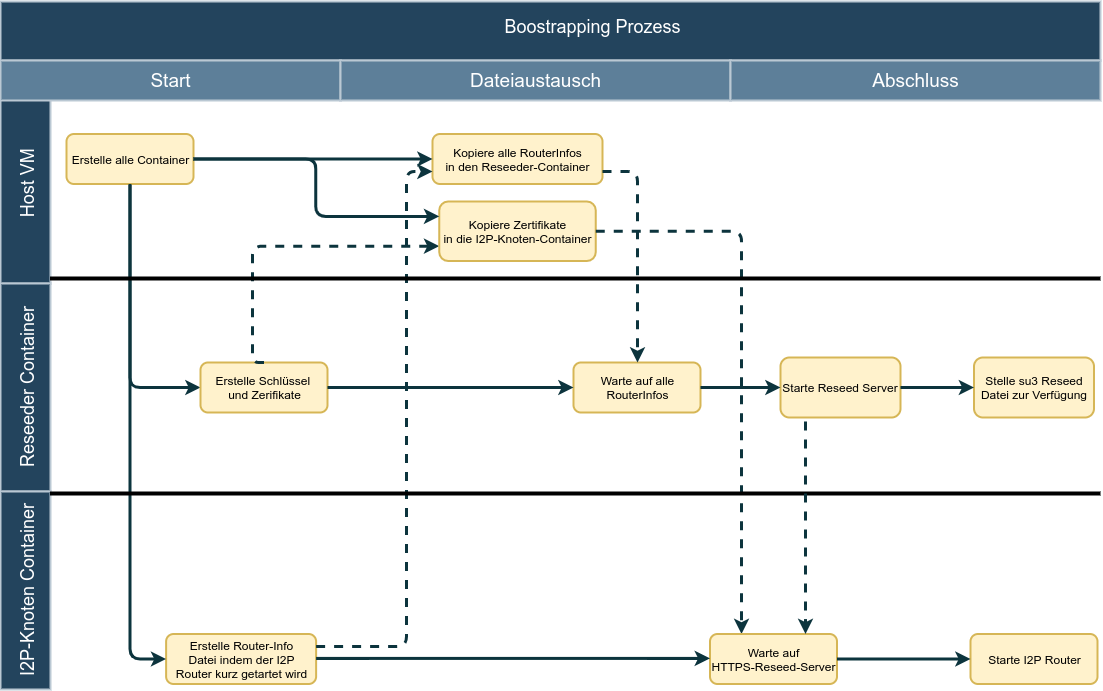
\includegraphics[height=0.85\textwidth]{bootstrap-diagram.png}
  \caption{Der Bootstrapping Prozess}\label{fig:bootstrap-diagram}
\end{figure*}
\end{landscape}% Landscape page


\subsection{Reproduzierbarkeit}

* Nix
* Pinning
    
\cite{noauthor_nixops_nodate-5}


\subsection{Isolieren}

Während unserer Tests wollen wir nur Traffic unserer eigenen Knoten im Netzwerk 

docker-compose respektive docker hat die option ein internes Netzwerk zu erstellen.

\subsubsection{Abgrenzen vom Haupt-Netzwerk}

Die Konfigurationsoption \lstinline|netid| erlaubt es die Netzwerknummer zu definieren.
Beim realen I2P-Netzwerk ist diese standardmässig auf \lstinline|2| gesetzt.

VM / Container, Konfigurationsoption \lstinline|nat|

Nix für container scheint nicht so gut zu funktionieren

Weil:

Das Builder der systemkonfigurationen inkl. der container getestet mit 100 konnte nicht durchlaufen da nix viel memory braucht (ich habe nach 16GB und 20min warten aufgehört da mein Laptop am swappen war)
Fehlerhafte netzwerkkonfiguration by default, falsche routen und ip konfigurationen (fehlende definition der netzwerkmaske)
Container selber sind unnötig gross


\subsection{I2Pd-Container}

Hauptsächlich wird in diesem Container der \lstinline|i2pd|-Prozess ausgeführt.
Um andere Knoten zu kontaktieren zu können muss dieser zu Beginn den Reseed-Container anfragen nach einer Liste von RouterInfos.

Der TCP-Client und TCP-Server sind ebenfalls in diesem Container angesiedelt.
Dies verletzt zwar das Prinzip, dass man nur einen Prozess in einem Docker-Container ausführen sollte,
jedoch ist das Ziel hiermit Messungenauigkeiten durch das Netzwerk, sowie die Netzwerkkonfiguration zu vereinfachen.

\subsection{Addressbuch}

%TODO: add to state of the art?

Standardmässig wird jeder i2pd-Destination eine b32-Adresse gegeben.
Diese Adresse wird abgeleitet vom Public-Key der generierten Destination.

Diese ist eine 52-Zeichen-lange aus kleinbuchstaben und zahlen bestehender Name um eine Destination zu adressieren. (z.b. \lstinline|b2cdodoyqg5v6go56bkaevvw777e2wyiflqh6zyyyxugy4cqlzuq.i2p|)

Zudem hat diese die Endung \lstinline|.i2p| damit klar ist, das dieser Name innerhalb des Overlaynetzwerks aufgelöst werden muss.

Diese ist jedoch nicht einfach zu handhaben und anstatt es ist einfacher die Knoten direkt anhand ihrer Nummer zu adressieren. Damit kann das Messskript vereinfacht werden, da es dieses dann nicht die 

Auch wird die Auswertung damit vereinfacht weil, der TCP-Client den verwendeten Namen des TCP-Servers auch in die Nachricht hineinpackt und der TCP-Server diesen als Messausgabe abspeichert.

Es wird beim Startvorgang des Netzwerks für jede erstellte destination für den TCP-Server ein Adressbucheintrag erstellt. Dieses Adressbuch ist eine einfache CSV-Datei wird wird 
im Bootstrapvorgang an alle Knoten verteilt.

Im falle von acht Knoten im Netzwerk sieht diese Datei beispielsweise so aus:

\begin{lstlisting}
tcpsrv-1.i2p,b2cdodoyqg5v6go56bkaevvw777e2wyiflqh6zyyyxugy4cqlzuq
tcpsrv-2.i2p,r6axddltht76mrtp5lrxtdxncilhgp7bcajkqtsj7l7fmoebgs3a
tcpsrv-3.i2p,ddhznqpxtgac7qa6yg6uzfpd55xoa2zfc4dwg4rh4qucx7veswlq
tcpsrv-4.i2p,3tyncnh7j4akqirrbdi4ek7nlysqmuvyav3ix326vwixvgoviz3q
tcpsrv-5.i2p,xj3qduyqur54v3mjgsxn6xa56q2ojyysf5n3bonpxyfxy5trnoja
tcpsrv-6.i2p,pt64eojrsvrp5w5izgwlide7j6vuw5td6g2pfrkurwsnmb4i7q2q
tcpsrv-7.i2p,aat6wqge3o7k2nabpwxrcu2vbbiydf3mj6n5k2zrrtozkrrpyfoa
tcpsrv-8.i2p,4wm4pqautqqb3a6yw3xif4zgwwu4v5tvpwv6onha27p5pkcqqepq
\end{lstlisting}

In der ersten Spalte ist der vereinfachte Name anzugeben und in der Zweiten Spalte die b32-Addresse, jedoch ohne die Endung \lstinline|.i2p|

\subsection{Der I2Pd-Prozess}

\subsubsection{TCP Server Tunnel}

Diese Tunnel-Konfiguration führt dazu, dass I2P eine neue Destination mit einer .b32-Addresse erstellt.

Mit der folgenden Tunnel-Konfigurations-Datei wird der \lstinline|i2pd| konfiguriert, um einen TCP-Server-Tunnel zur Verfügung zu stellen:
\begin{lstlisting}
# serve some tcp service to others in the network
[tcp-in]
type = server
host = 127.0.0.1
port = 2323
keys = tcp-in.dat
gzip = false
enableuniquellocal = true
\end{lstlisting}

Hierbei gilt es zu beachten, das die Schlüssel angegeben mit der \lstinline|keys|-Option, beim Aufstarten generiert werden.
Auch wurde mittels der Option \lstinline|gzip| die Komprimierung-Deaktiviert, damit auch wirklich die richtigen Nachrichten-Grössen übermittelt werden.
Die Option\lstinline|enableuniquellocal| wurde noch aktiviert, um die Auswertung zu vereinfachen. Denn diese führt dazu das der TCP-Server nicht immer dieselbe Ausgangsadresse \lstinline|127.0.0.1| bekommt, sondern je nach Sender der Nachricht eine andere \lstinline|127.0.0.0/8|-Adresse anhand der ersten Bytes des Public-Keys erhält.

%TODO: Reference config, especiallfor for enableuniquellocal.

\subsection{Nachrichten}

Die darüberliegende Blockchain-Schicht von diva.exchange versendet mittels eines Gossip-Protokolls die neuen Blocks der Blockchain an alle Knoten.
%TODO: add gossip protocol to glossary
Diese 64Kb grossen Blocks werden über eine Web-Socket-Verbindung an die Nachbarknoten übermittelt.
Die Nachbarknoten leiten diese dann wieder weiter an ihre jeweiligen Nachbarknoten.
Dieser Prozess wird solange wiederholt bis alle Knoten im Netzwerk den neuen Block erhalten haben.

Nach Absprache mit dem Auftraggeber wird dies im Testnetzwerk mittels versenden von TCP-Nachrichten nachgestellt.
Bei Web-Sockets handelt es sich vereinfacht ausgedrückt wiederum um eine TCP-ähnliche Verbindung über HTTP. HTTP selber TCP auch als Transportschicht.


\begin{itemize}
    \item Originator Node Id
    \item Destination Address
    \item Grösse der versendeten Nachricht in Bytes
    \item Zeitpunkt in nanosekunden seit 1.1.1970 
\end{itemize}

\subsection{Nachrichten-Log}


\subsubsection{Socks5-Proxy für den TCP-Client}

Dieser Socks5-Proxy ist der Gateway um innerhalb des I2P-Overlaynetzwerk zu kommunizieren.

Der folgende Ausschnitt aus der \lstinline|i2pd.conf| zeigt auf wie der Socks5-Proxy konfiguriert wurde:

\begin{lstlisting}
[socksproxy]
## Uncomment and set to 'false' to disable SOCKS Proxy
enabled = true
## Address and port service will listen on, like 127.0.0.1
address = 127.0.0.1
port = 4445
\end{lstlisting}

\subsection{TCP-Server}


\subsection{TCP-Client}

Damit der TCP-Client in das I2P-Overlaynetzwerk verbinden kann muss dieser fähig sein mit einem Socks5-Proxy zu kommunizieren.



\section{Testing}

CI? most don't allow this...

have a machine to deploy to

\subsection{BATS-Tests}

Diese Tests sind im Verzeichnis \lstinline|tests/| in der \lstinline|i2p-testnet|-Repository zu finden.

Um schnell zu prüfen ob das Netzwerk korrekt konfiguriert wurde gibt es das Test-Modul \lstinline|tests/networking.bats|.

\subsection{CI für den Bericht}

Da der Bericht mit Hilfe von \LaTex umgesetzt wurde, verhält sich dieser 

\section{Benutzerhandbuch}

Dieser Abschnitt erklärt wie ein Tester selber neue Testnetzwerke erstellen, die Tests-Konfigurieren und selber

\subsection{Deployment der Test-VM}

Für genauere Anweisungen und weitere Möglichkeiten welche durch nixops geboten werden, siehe das ``NixOps User's Guide''\footnote{\url{https://releases.nixos.org/nixops/nixops-1.5/manual/manual.html}}.


\subsection{Konfiguration einer Messung}

\subsection{Ausführen einer Messung}
